%% CV - Álvaro López Álvarez
%% Tailored for: Junior Backend Engineer - Lending (Financial Empowerment) - N26
%%
%% Compile with: lualatex main_n26_en.tex
%% (pdflatex often fails on modern MiKTeX with fontawesome5 font-expansion errors.)

\documentclass[11pt,a4paper,sans]{moderncv}
\moderncvstyle{banking}
\moderncvcolor{blue}

% Force both first and last name AND section headings to render in moderncv
% blue (color1). Default banking on lualatex+MiKTeX leaves these black, which
% looks inconsistent with the rest of the blue accent scheme.
\renewcommand*{\firstnamestyle}[1]{{\fontsize{34}{36}\bfseries\upshape\color{color1}#1}}
\renewcommand*{\lastnamestyle}[1]{{\fontsize{34}{36}\bfseries\upshape\color{color1}#1}}
\renewcommand*{\sectionstyle}[1]{{\sectionfont\color{color1}#1}}

\usepackage[utf8]{inputenc}
\usepackage{hyperref}
\usepackage{needspace}
\hypersetup{
    colorlinks=true,
    linkcolor=blue,
    filecolor=magenta,
    urlcolor=blue,
    pdftitle={Álvaro López Álvarez - CV - N26},
    pdfpagemode=FullScreen,
}
\usepackage[scale=0.75]{geometry}
\usepackage{import}
\usepackage{eso-pic}

% personal data
\name{Álvaro}{López Álvarez}
\address{Valencia, España}{}{}
\phone[mobile]{+34 640764553}
\email{alvaro.lopez.dev@gmail.com}
\extrainfo{\href{https://www.linkedin.com/in/alvarolopez-dev}{LinkedIn}, \href{https://github.com/alerone}{GitHub}, \href{https://alerone.github.io/portfolio}{Portfolio}}

% moderncv's banking style (head variant 3) does not wire up \photo at all -
% it is silently ignored. Overlay the photo directly instead, anchored to the
% page corner so it is independent of the centered banking header layout.
\AddToShipoutPictureFG{%
  \ifnum\value{page}=1
    \AtPageUpperLeft{%
      \hspace*{\dimexpr\paperwidth-2.3cm-1.3cm\relax}%
      \raisebox{\dimexpr-1.3cm-2.3cm\relax}{\fboxsep0pt\fboxrule0.6pt\fcolorbox{color1}{white}{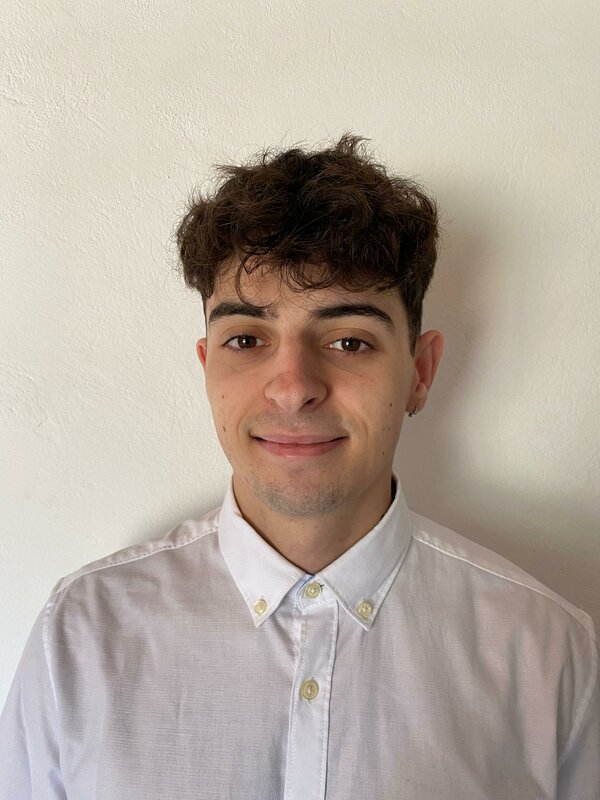
\includegraphics[width=2.3cm]{photo}}}%
    }%
  \fi
}

\begin{document}

\makecvtitle

% ============================================================
%     PROFILE STATEMENT
% ============================================================

\vspace{6pt}
\small{Junior Software Engineer building Java backend fundamentals through a self-directed Spring Boot and Apache Kafka project (in progress), plus Kotlin experience from native Android development. Used to working independently and owning problems end to end, evidenced by an R\&D role designing an autonomous agent that resolves data-access policy without supervision. Complements this with two full-stack roles at ITI (Go, React/TypeScript), Docker containerization, and CI/CD via GitHub Actions. A consistent pattern of learning new stacks independently and getting things done, from the Kafka-based ticketing platform to a from-scratch HTTP/1.1 server.}

% ============================================================
%     CORE COMPETENCIES
% ============================================================

\section{Core Competencies}
\vspace{1pt}
\begin{itemize}

\item \textbf{Java \& Kotlin Development}: Spring Boot, JPA/Hibernate, JUnit; Kotlin via native Android (MVVM) development

\item \textbf{Event-Driven \& Distributed Systems}: Apache Kafka, Docker, microservices, NATS JetStream

\item \textbf{Backend Fundamentals}: REST API design, PostgreSQL, OAuth 2.0/JWT

\item \textbf{Autonomous Delivery}: independent feature ownership, self-managed R\&D projects, agentic/LLM tooling

\item \textbf{Full-Stack Complement}: Golang, TypeScript/JavaScript (React)

\end{itemize}

% ============================================================
%     PROFESSIONAL EXPERIENCE
% ============================================================

\section{Professional Experience}
\vspace{3pt}
\begin{itemize}

% --- Most Recent Role ---
\needspace{5\baselineskip}
\item{\cventry{Feb 2026--Jun 2026}{R\&D Developer}{Instituto Tecnológico de Informática (ITI)}{Valencia, España}{}{\vspace{1pt}
\begin{itemize}
    \item Implemented LLM-based improvements to a search engine
    \item Built an autonomous multi-step agent converting natural-language questions into validated, read-only SQL queries against a PostgreSQL schema, including safety validation and error-driven retries, run independently with minimal day-to-day oversight
    \item Managed scope and delivery priorities on a production-adjacent data-governance platform, prioritizing schema selection and safety validation first as the specification evolved
\end{itemize}}}

\vspace{3pt}

% --- Previous Role ---
\needspace{5\baselineskip}
\item{\cventry{Feb 2024--Jun 2024}{Full-Stack Developer Intern}{Instituto Tecnológico de Informática (ITI)}{Valencia, España}{}{\vspace{1pt}
\begin{itemize}
    \item Developed and maintained a business-critical corporate personnel management application (Intranet)
    \item Implemented new frontend features using React and TypeScript, improving internal usability
    \item Collaborated with frontend and backend engineers on backend development, ensuring smooth integration between services via version-controlled Git workflows
\end{itemize}}}

\end{itemize}

% ============================================================
%     SELECTED PROJECTS
% ============================================================

\section{Selected Projects}
\vspace{1pt}
\begin{itemize}

\needspace{3\baselineskip}
\item \textbf{Kafka + Spring Boot Ticketing Platform} (in progress): Self-directed project building event-driven microservices (reservation, payment, notification, audit) with Spring Boot 3 and Apache Kafka to learn producer/consumer patterns and event-driven microservice design.

\needspace{3\baselineskip}
\item \textbf{ValenMove}: Native Android app (Kotlin, MVVM) unifying Valencia's public transport into one interface; reverse-engineered public APIs for real-time data. Final Degree Project, grade 9/10.

\needspace{3\baselineskip}
\item \textbf{English Learning API}: Spring Boot REST API with JPA entities, DTOs/mappers, Jakarta validation, centralized error handling, and randomized practice challenges with attempt tracking.

\needspace{3\baselineskip}
\item \textbf{HTTP from TCP (Java)}: Java re-implementation of an HTTP/1.1 server directly on raw sockets, built to deepen Java fundamentals: I/O, concurrency via executors, JUnit testing.

\end{itemize}

% ============================================================
%     EDUCATION
% ============================================================

\needspace{9\baselineskip}
\section{Education}
\vspace{1pt}
\begin{itemize}

\needspace{4\baselineskip}
\item{\cventry{2024--2026}{Master's Degree in Computer Engineering (MUIINF)}{Polytechnic University of Valencia (UPV)}{Valencia, España}{}{\vspace{1pt}
In progress (expected Sep 2026). Topics: distributed systems, high-performance computing, cybersecurity, embedded systems.
}}

\vspace{3pt}

\needspace{4\baselineskip}
\item{\cventry{2020--2024}{Grado (BSc) in Ingeniería Informática, Software Engineering track}{Polytechnic University of Valencia (UPV)}{Valencia, España}{}{\vspace{1pt}
GPA: 8.88/10. Thesis: ``ValenMove - Unified Public Transport App'' (grade 9/10).
}}

\end{itemize}

% ============================================================
%     LANGUAGES
% ============================================================

\section{Languages}
\vspace{1pt}
\begin{itemize}
\item Spanish (native), Catalan (native), English (B2, confident conversational).
\end{itemize}

% ============================================================
%     REFERENCES
% ============================================================

\section{References}
\vspace{1pt}
\begin{itemize}
\item{Available upon request.}
\end{itemize}

\end{document}
